\documentclass{beamer}
\setbeamerfont{headline}{size=\footnotesize}

\mode<presentation>{
\usetheme{Montpellier}
\setbeamercovered{transparent}
\usecolortheme{lsc}
}

\mode<handout>{
  % tema simples para ser impresso
  \usepackage[bar]{beamerthemetree}
   % Colocando um fundo cinza quando for gerar transparências para serem impressas
  % mais de uma transparência por página
  \beamertemplatesolidbackgroundcolor{black!5}
}

\usepackage{fancyvrb}

\usepackage{amsmath,amssymb}
\usepackage[brazil]{varioref}
\usepackage[english,brazil]{babel}
\usepackage[utf8]{inputenc}
\usepackage{fontawesome}

\usepackage{makecell} % Adicione isso no preâmbulo do documento

%\usepackage[latin1]{inputenc}
\usepackage{graphicx}
\usepackage{listings}
\usepackage{url}
\usepackage{colortbl}
\usepackage{caption}
\usepackage{tikz}
\usepackage{transparent}
\usepackage{multirow}
\usepackage{graphicx}
\usepackage{listings}
\usepackage{exercise,chngcntr}

\usepackage{listings}
\usepackage{xcolor}
\usepackage{tikz}
\usetikzlibrary{shapes, arrows.meta, positioning}


% Definição de cores para o código Python
\definecolor{codegreen}{rgb}{0,0.6,0}
\definecolor{codegray}{rgb}{0.5,0.5,0.5}
\definecolor{codepurple}{rgb}{0.58,0,0.82}
\definecolor{backcolour}{rgb}{0.95,0.95,0.92}
% Configuração do estilo do código Python
\lstdefinestyle{mystyle}{
    xleftmargin=0pt,           % Aumenta a margem esquerda
    xrightmargin=10pt,          % Aumenta a margem direita
    frame=single,               % Adiciona um quadro ao redor do código
    framesep=10pt,              % Espaço entre o quadro e o código
    % Outras configurações do lstlisting...
    backgroundcolor=\color{backcolour},
    commentstyle=\color{codegreen},
    keywordstyle=\color{magenta},
    numberstyle=\tiny\color{codegray},
    stringstyle=\color{codepurple},
    basicstyle=\footnotesize\ttfamily,
    breakatwhitespace=false,
    breaklines=true,
    captionpos=b,
    keepspaces=true,
    %numbers=left,
    numbersep=5pt,
    showspaces=false,
    showstringspaces=false,
    showtabs=false,
    tabsize=2,
    basicstyle=\ttfamily, % Usa uma fonte de largura fixa para o código
    upquote=true,         % Tenta usar aspas retas se a fonte suportar,
    breakatwhitespace=false, % Quebra linhas em espaços em branco quando possível
}

\lstset{style=mystyle}


\beamertemplatetransparentcovereddynamic
\addtobeamertemplate{title page}{\centering{ 
\includegraphics[width=1.25cm]{figs/logo.png}}}{}
\title[]{Visão Computacional}
\author[Elton Sarmanho]{ 
Professor: Elton Sarmanho\inst{1} 
\newline
E-mail: \href{mailto:eltonss@ufpa.br}{eltonss@ufpa.br}\newline
\href{https://github.com/eltonsarmanho}{\faGithub} \href{https://www.linkedin.com/in/elton-sarmanho-836553185/}{\faLinkedinSquare}
}   
  \institute[UFRailwayPA]{
   \inst{1}%
     Faculdade de Sistemas de Informação - UFPA/CUNTINS
     }     
 
% Se comentar a linha abaixo, irá aparecer a data quando foi compilada a apresentação  
\date{\today}
\pgfdeclareimage[height= 1.25 cm]{inf}{figs/logo.png}
% pode-se colocar o LOGO assim
\logo{{\transparent{0.35}\pgfuseimage{inf}}}

% \AtBeginSection[]{
%   \begin{frame}<beamer>
%     \frametitle{Roteiro}
%     \tableofcontents[currentsection,currentsubsection]
%   \end{frame}  
% }

\setbeamertemplate{navigation symbols}{\insertframenavigationsymbol \insertsectionnavigationsymbol \insertbackfindforwardnavigationsymbol} 


\expandafter\def\expandafter\insertshorttitle\expandafter{%
  \insertshorttitle\hfill%
  \insertframenumber\,/\,\inserttotalframenumber}
  \renewcounter{Exercise}[section]
  \newcounter{Example}



\begin{document}

\setbeamertemplate{logo}{}
\begin{frame}
\titlepage
\end{frame}
%Começar mostrar Logo apos slide de titulo
\logo{{\transparent{0.35}\pgfuseimage{inf}}}

\begin{frame}
\frametitle{Roteiro}
\tableofcontents[sections={1-3}]
\end{frame}


%Declaração das Imagens da Apresentação

%%%%%%%%%%%%%%%%%%%%%%%%%%%%%%%%%%%%%%%%
\section{Planejamento}

\begin{frame}
Nesta aula:

\begin{itemize}
 \item Vamos explorar os conceitos fundamentais de Visão Computacional.
 \item Ter panorama sobre conceito.
 \item Reconhecimento de Gestos
 \item Códigos do Professor estão no github
\end{itemize}


\end{frame}

\section{Introdução}
\begin{frame}
\frametitle{O que é Visão Computacional?}
\begin{itemize}
    \item A visão computacional é um canal perceptual que processa estímulos visuais para criar uma representação do mundo.
    \item A diferença entre visão humana e computacional:
    \begin{itemize}
        \item Visão Humana: Utiliza sensores passivos, como os olhos.
        \item Visão Computacional: Alguns sistemas usam sensores ativos (ex: radar, ultrassom).
    \end{itemize}
    \item Uso de algoritmos e representações que permitem
uma máquina reconhecer objetos, cenas, pessoas e
atividades (percepção e interpretação)
\end{itemize}
\end{frame}


\begin{frame}
\frametitle{O que é Visão Computacional?}
\begin{itemize}
    \item A visão computacional é um canal perceptual que processa estímulos visuais para criar uma representação do mundo.
    \item A diferença entre visão humana e computacional:
    \begin{itemize}
        \item Visão Humana: Utiliza sensores passivos, como os olhos.
        \item Visão Computacional: Alguns sistemas usam sensores ativos (ex: radar, ultrassom).
    \end{itemize}

     \begin{figure}
 \centering
 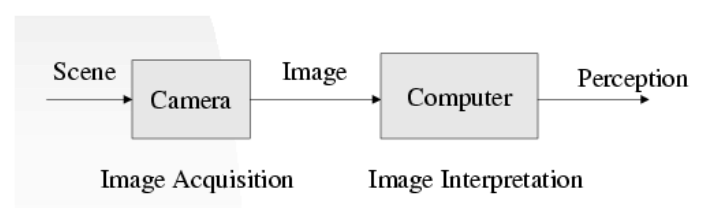
\includegraphics[width=0.8\textwidth]{figs/visao.png} \end{figure}
\end{itemize}
\end{frame}

\begin{frame}{Utilidades da visão computacional}
    \begin{itemize}
        \item O crescimento no volume de imagens geradas amplia suas possíveis aplicações:
        \begin{itemize}
            \item Automatizar tarefas repetitivas e tediosas
            \item Aperfeiçoar a interação entre humanos e computadores
            \item Fornecer capacidades de percepção para robôs e sistemas autônomos
            \item Facilitar a organização e o acesso a informações visuais
        \end{itemize}
        \item Metas principais:
        \begin{itemize}
            \item Permitir que máquinas compreendam cenários visuais
            \item Apoiar o desenvolvimento de dispositivos para pessoas com deficiência visual
            \item Automatizar processos de análise e visualização de imagens
        \end{itemize}
    \end{itemize}
\end{frame}

\begin{frame}{Para que serve a visão computacional?}
     \begin{figure}
 \centering
 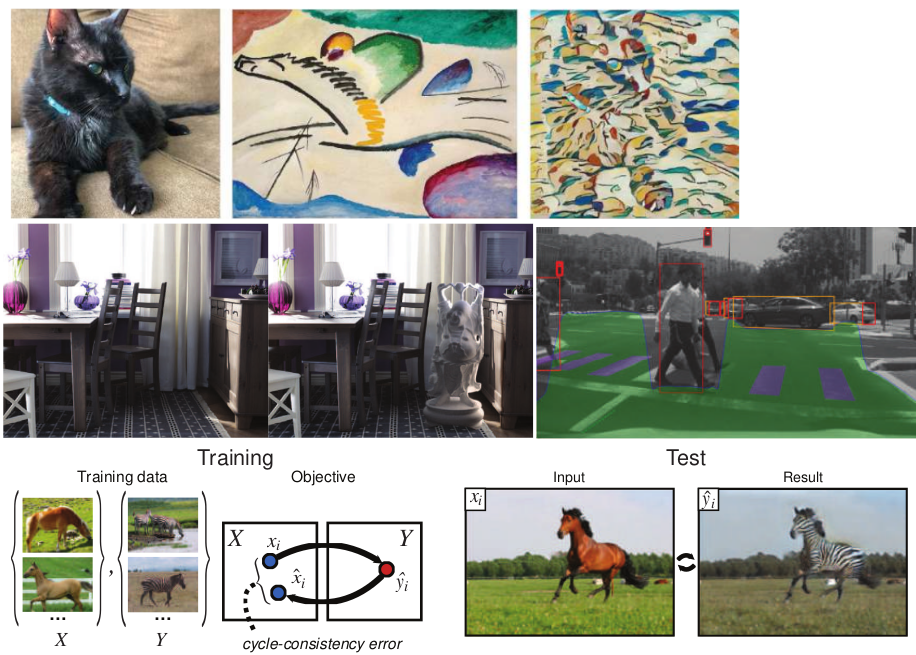
\includegraphics[width=0.8\textwidth]{figs/ExemplosVisao.png} \end{figure}
\end{frame}
\section{Aplicações}

\begin{frame}{Aplicações}
    \begin{itemize}
        \item Análise de imagens médicas
        \item Manipulação de Imagens
        \item Segurança: biometria, monitoramento, localização
        \item Multimídia e Educação
        \item Reconhecimento de Padrões
        \item Realidade aumentada
        \item Reconhecimento de Objetos
        \item Efeitos visuais
    \end{itemize}
\end{frame}

\begin{frame}{Análise de imagens médicas}
   \begin{figure}
 \centering
 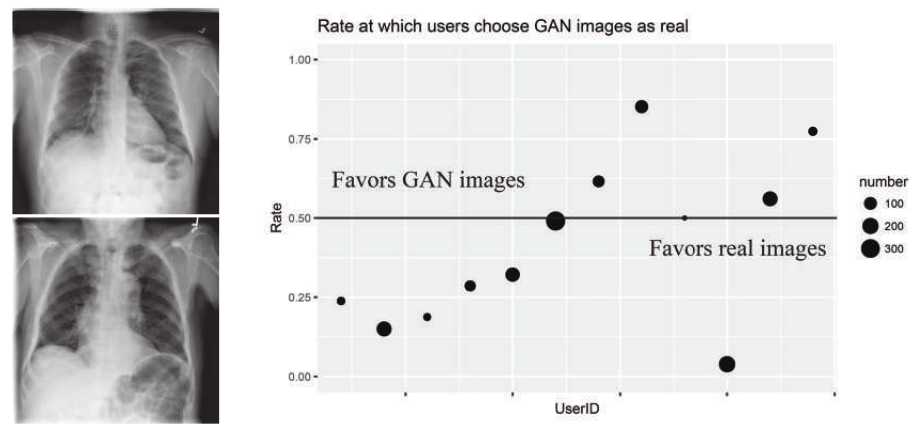
\includegraphics[width=0.8\textwidth]{figs/AnaliseMedica.png} \end{figure}
\end{frame}

\begin{frame}{Manipulação de Imagens - Style transfer}
   \begin{figure}
 \centering
 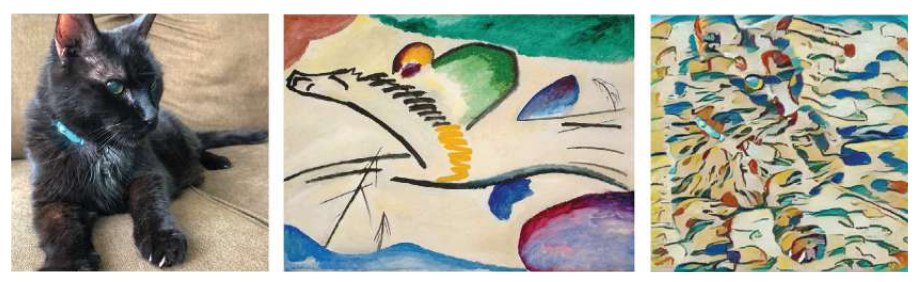
\includegraphics[width=0.8\textwidth]{figs/StyleTransfer.png} \end{figure}
\end{frame}

\begin{frame}{Segurança: monitoramento corporal}
   \begin{figure}
 \centering
 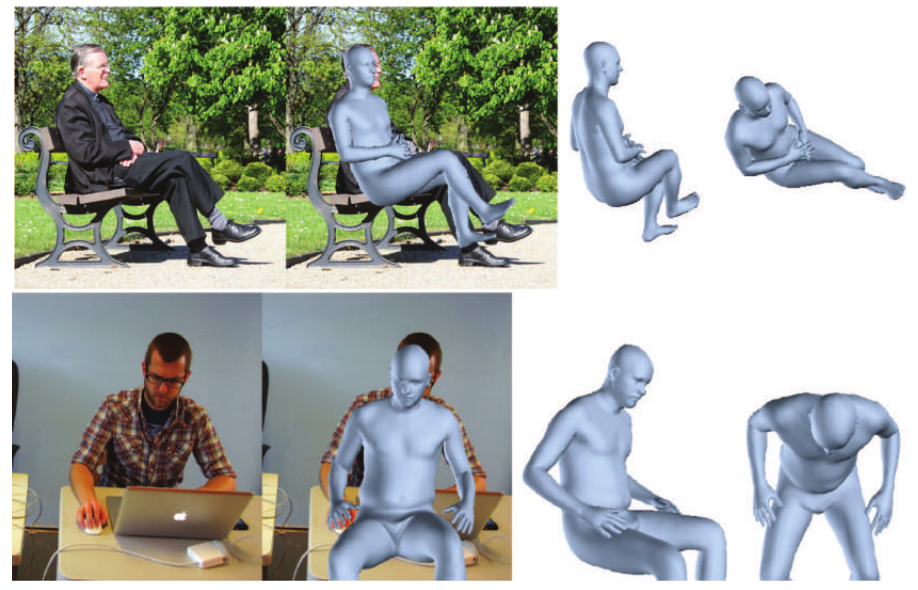
\includegraphics[width=0.8\textwidth]{figs/Seguranca.png} \end{figure}
\end{frame}

\begin{frame}{Segurança: Pedestres e veículos}
   \begin{figure}
 \centering
 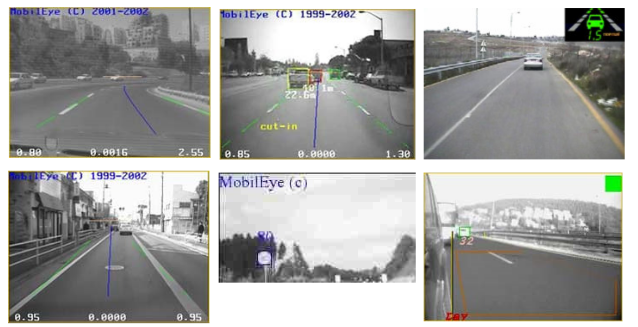
\includegraphics[width=0.9\textwidth]{figs/Seguranca2.png} \end{figure}
\end{frame}


\begin{frame}{Multimídia e Educação}
   \begin{figure}
 \centering
 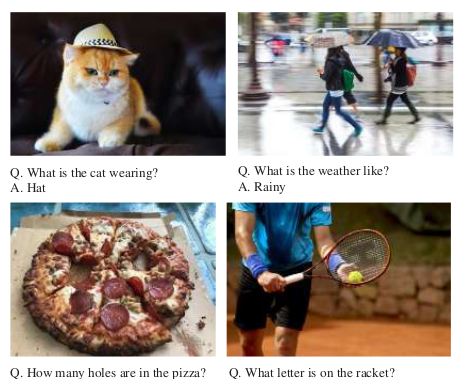
\includegraphics[width=0.75\textwidth]{figs/QA.png} \end{figure}
\end{frame}

\begin{frame}{Reconhecimento de Padrões}
   \begin{figure}
 \centering
 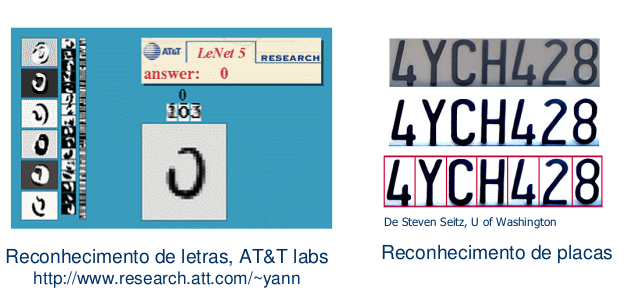
\includegraphics[width=1\textwidth]{figs/ReconhecimentoPadroes.png}
 \end{figure}
\end{frame}

\begin{frame}{Realidade aumentada}
   \begin{figure}
 \centering
 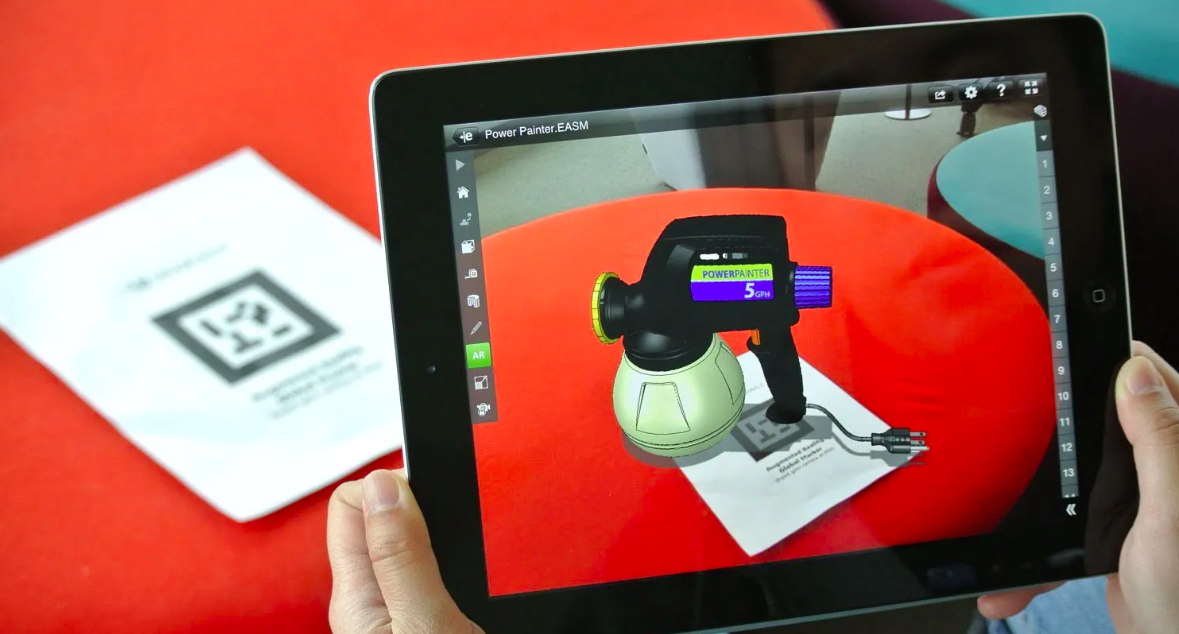
\includegraphics[width=1\textwidth]{figs/RV.png}
 \end{figure}
\end{frame}

\begin{frame}{Reconhecimento de Objetos}
   \begin{figure}
 \centering
 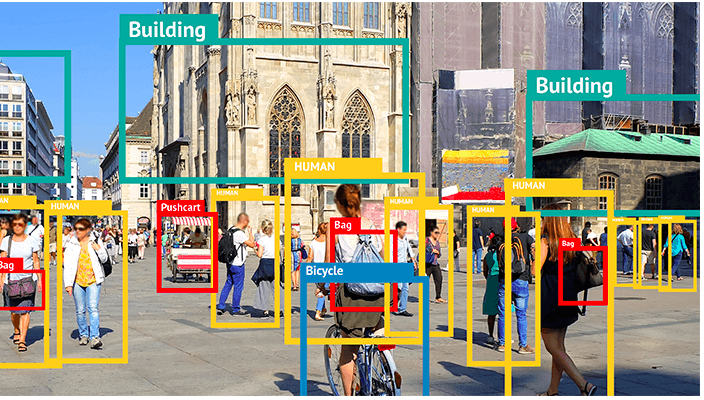
\includegraphics[width=1\textwidth]{figs/ReconhecimentoObjetos.png}
 \end{figure}
\end{frame}

\begin{frame}{Efeitos Visuais}
   \begin{figure}
 \centering
 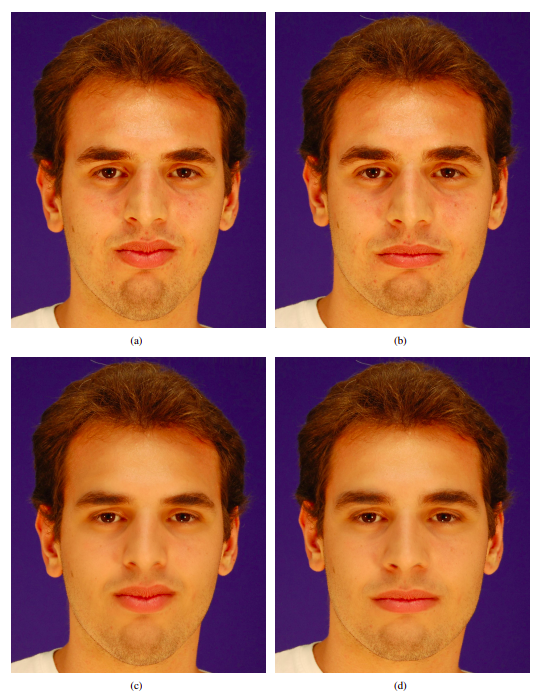
\includegraphics[width=0.5\textwidth]{figs/EfeitosVisuais.png}
 \end{figure}
\end{frame}

\section{Desafios}

\begin{frame}{Desafios}
    \begin{itemize}
        \item Por que é um desafio?
        \begin{itemize}
            \item A relação entre dados visuais e o mundo real não é direta:
            \begin{itemize}
                \item Uma mesma superfície pode apresentar uma ampla variedade de materiais, condições de iluminação e formas geométricas.
            \end{itemize}
            \item Processamento de imagens é intensivo em recursos computacionais.
            \item A principal dificuldade: ainda não compreendemos plenamente o problema!
        \end{itemize}
    \end{itemize}
\end{frame}

\begin{frame}{Reconhecimento de Padrões em Imagens}
    \begin{itemize}
        \item Considere o desafio de identificar uma parede de tijolos em imagens.
        \item Uma pesquisa visual pode retornar exemplos variados:
        \begin{itemize}
            \item Diferentes estilos e texturas de tijolos.
            \item Presença de objetos ou texto sobrepostos.
            \item Variações nas condições de iluminação e perspectiva.
        \end{itemize}
        \item Essas diferenças ilustram as dificuldades no reconhecimento de padrões visuais.
    \end{itemize}
  \begin{figure}
 \centering
 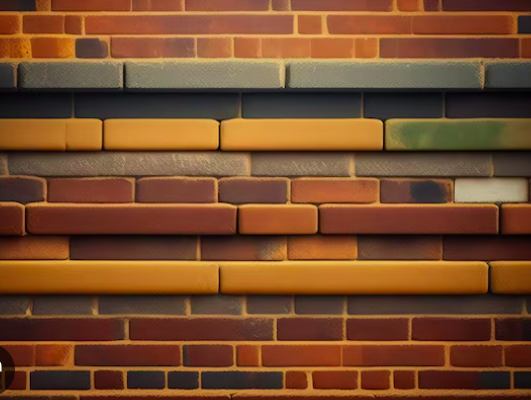
\includegraphics[width=0.4\textwidth]{figs/Tijolos.png}
 \end{figure}
\end{frame}



\begin{frame}{Desafios da Visão Computacional: Iluminação}
    \begin{itemize}
        \item \textbf{Impacto da iluminação na análise de imagens:}
        \begin{itemize}
            \item Condições de iluminação podem alterar drasticamente a aparência de objetos e cenas.
            \item Diferenças de sombra, brilho e contraste dificultam a consistência na detecção e reconhecimento de padrões.
        \end{itemize}
        \item \textbf{Problemas comuns causados pela iluminação:}
        \begin{itemize}
            \item Ambientes mal iluminados podem esconder detalhes.
            \item Reflexos excessivos podem distorcer características visuais.
            \item Mudanças na intensidade da luz alteram cores percebidas.
        \end{itemize}
    \end{itemize}
    \begin{center}
        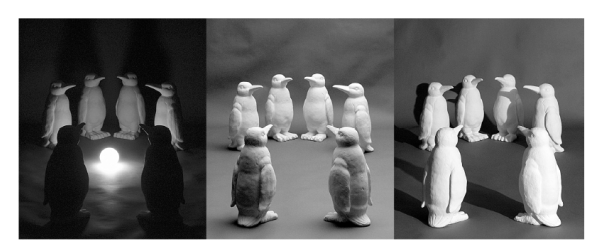
\includegraphics[width=0.8\textwidth]{figs/iluminacao.png} % Adicione uma imagem ilustrativa, se possível.
    \end{center}
\end{frame}

\begin{frame}{Desafios da Visão Computacional: Iluminação}
    \begin{itemize}

        \item \textbf{Soluções e estratégias:}
        \begin{itemize}
            \item Uso de algoritmos robustos à variação de iluminação, como normalização de intensidade.
            \item Técnicas de aprendizado profundo (deep learning) para generalizar sob diferentes condições de luz.
            \item Sensores de luz adaptativos para capturar detalhes relevantes mesmo em ambientes desafiadores.
        \end{itemize}
    \end{itemize}
    \begin{center}
        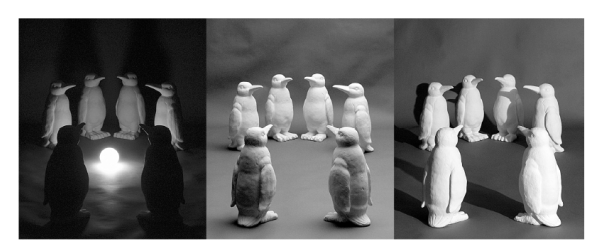
\includegraphics[width=0.8\textwidth]{figs/iluminacao.png} % Adicione uma imagem ilustrativa, se possível.
    \end{center}
\end{frame}

\begin{frame}{Desafios da Visão Computacional: Oclusão}
    \begin{itemize}
        \item \textbf{O que é oclusão?}
        \begin{itemize}
            \item Acontece quando partes de objetos ou cenas ficam ocultas devido à sobreposição de elementos no campo de visão.
        \end{itemize}

    \end{itemize}
    \begin{center}
        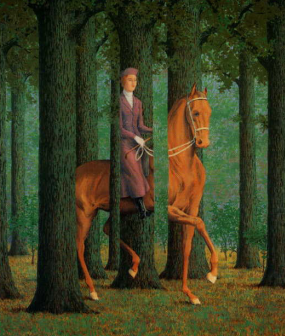
\includegraphics[width=0.4\textwidth]{figs/oclusao.png} % Adicione uma imagem ilustrativa, se possível.
    \end{center}
\end{frame}


\begin{frame}{Desafios da Visão Computacional: Oclusão}
    \begin{itemize}

        \item \textbf{Impacto da oclusão:}
        \begin{itemize}
            \item Reduz a informação disponível, dificultando a identificação de objetos.
            \item Pode levar a erros no reconhecimento ou segmentação de partes de uma imagem.
            \item Exige que o sistema "imagine" ou reconstrua elementos ausentes com base em dados incompletos.
        \end{itemize}

        \end{itemize}

    \begin{center}
        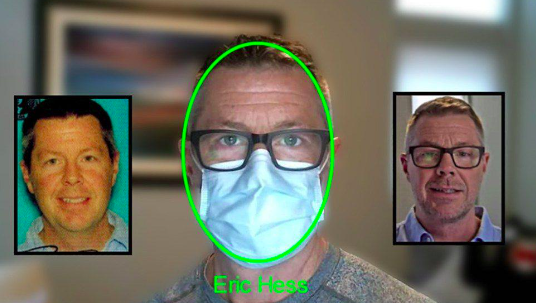
\includegraphics[width=0.5\textwidth]{figs/oclusao2.png} % Adicione uma imagem ilustrativa, se possível.
    \end{center}
\end{frame}


\begin{frame}{Desafios da Visão Computacional: Oclusão}
    \begin{itemize}

        \item \textbf{Soluções e abordagens:}
        \begin{itemize}
            \item Uso de redes neurais para inferir partes ocultas de objetos com base em padrões aprendidos.
            \item Técnicas de visão multivista (imagens de diferentes ângulos) para reconstruir informações ocluídas.
            \item Modelos probabilísticos para prever as características de áreas ocultas.
        \end{itemize}
        \item \textbf{Exemplo prático:}
        \begin{itemize}
            \item Reconhecer um rosto parcialmente coberto por óculos, máscara ou outro objeto.
        \end{itemize}
    \end{itemize}

\end{frame}


\begin{frame}{Desafios da Visão Computacional: Escala}
    \begin{itemize}
        \item \textbf{O que é o desafio da escala?}
        \begin{itemize}
            \item Refere-se à dificuldade de identificar e reconhecer objetos em tamanhos diferentes dentro de uma imagem ou vídeo.
            \item Objetos podem parecer menores ou maiores dependendo da distância ou da perspectiva.
        \end{itemize}

    \end{itemize}
     \begin{center}
        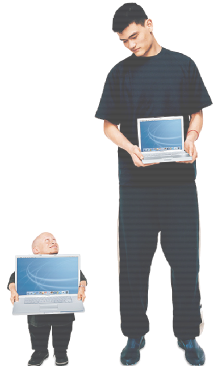
\includegraphics[width=0.2\textwidth]{figs/escala.png} % Adicione uma imagem ilustrativa, se possível.
    \end{center}
\end{frame}


\begin{frame}{Desafios da Visão Computacional: Escala}
    \begin{itemize}

        \item \textbf{Impacto da escala:}
        \begin{itemize}
            \item Dificulta o reconhecimento, especialmente em cenários onde o mesmo objeto aparece em tamanhos variados.
            \item Complica tarefas de segmentação e detecção devido à falta de proporção constante.
            \item Afeta algoritmos que não são invariantes a mudanças de escala.
        \end{itemize}
        \item \textbf{Abordagens para lidar com escala:}
        \begin{itemize}
            \item Uso de técnicas invariantes à escala, como SIFT (Scale-Invariant Feature Transform).
            \item Redes neurais convolucionais (CNNs) com camadas que aprendem múltiplos níveis de detalhe.
            \item Análise multiresolução para capturar padrões em diferentes tamanhos.
        \end{itemize}

    \end{itemize}

\end{frame}


\begin{frame}{Desafios da Visão Computacional: Escala}
    \begin{itemize}


        \item \textbf{Exemplo prático:}
        \begin{itemize}
            \item Reconhecimento de veículos em uma estrada, onde carros próximos e distantes aparecem em escalas diferentes.
        \end{itemize}
    \end{itemize}
     \begin{center}
        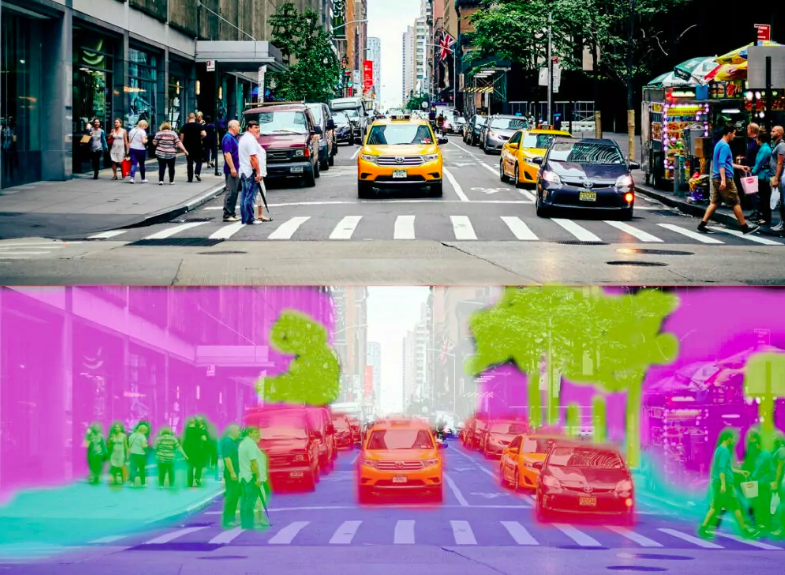
\includegraphics[width=0.5\textwidth]{figs/escala2.png} % Adicione uma imagem ilustrativa, se possível.
    \end{center}
\end{frame}


\subsection{Questões críticas}

\begin{frame}{Questões críticas}
    \begin{itemize}
        \item Qual informação deve ser extraída da imagem?
        \item Como a informação pode ser extraída?
        \item Como a informação deve ser representada?
        \item Como a informação pode ser usada para análise e entendimento?
    \end{itemize}
\end{frame}

\begin{frame}{Como os computadores vêem?}
\begin{center}
        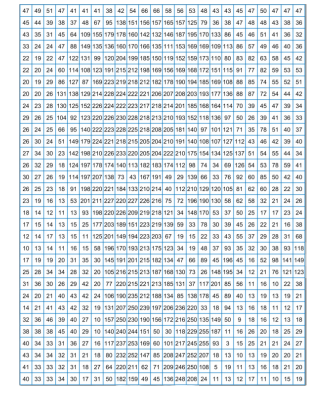
\includegraphics[width=0.5\textwidth]{figs/matriz.png} % Adicione uma imagem ilustrativa, se possível.
    \end{center}
\end{frame}


\begin{frame}{Como os computadores vêem?}
\begin{center}
        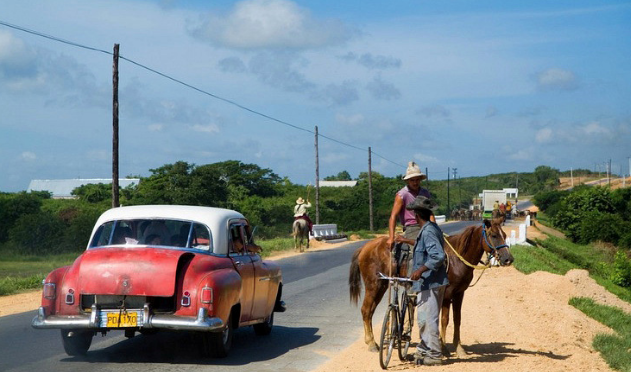
\includegraphics[width=0.9\textwidth]{figs/imagem_alto_nivel.png} % Adicione uma imagem ilustrativa, se possível.
    \end{center}
\end{frame}
\begin{frame}{Como os computadores vêem?}
\begin{center}
        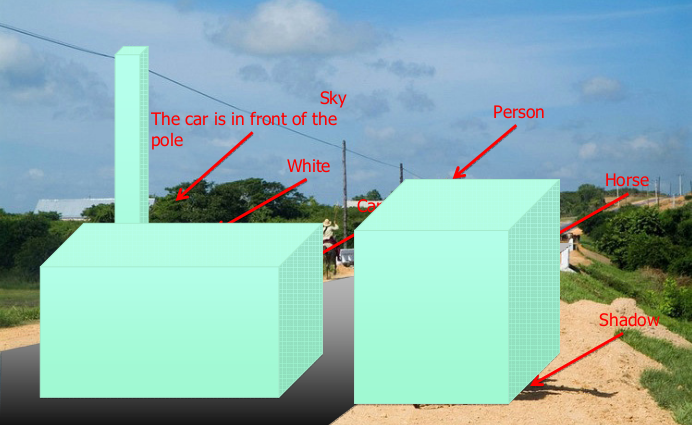
\includegraphics[width=0.9\textwidth]{figs/imagem_alto_nivel_2.png} % Adicione uma imagem ilustrativa, se possível.
    \end{center}
\end{frame}

\begin{frame}{Reconhecimento}
    \begin{itemize}
        \item Como diferentes atributos, como cor, textura, formato e movimento, podem contribuir para o reconhecimento de padrões?
        \begin{itemize}
            \item Quais partes de uma imagem devem ser analisadas conjuntamente?
            \item É possível identificar objetos sem se concentrar em detalhes específicos?
            \item Como reconhecer objetos que possuem muitos parâmetros variáveis?
            \item Qual é a melhor forma de organizar um banco de dados para modelos de objetos?
        \end{itemize}
    \end{itemize}
\end{frame}

\subsection{Cor}
\begin{frame}{Introdução à Cor}
    \begin{itemize}
        \item A cor é um sinal visual fundamental usado por humanos e máquinas para interpretar o mundo.
        \item Humanos percebem cores baseados em três receptores sensíveis a diferentes comprimentos de onda.
        \item Sistemas de câmera replicam essa percepção usando três tipos de sensores: RGB.
    \end{itemize}
\end{frame}

\begin{frame}{Visão Humana e Tricromacia}
    \begin{itemize}
        \item A visão humana funciona pela comparação das respostas dos três tipos de receptores na retina.
        \item Princípio da tricromacia:
        \begin{itemize}
            \item Cores percebidas podem ser combinadas usando três primárias (vermelho, verde, azul - RGB).
        \end{itemize}
        \item Este conceito permite representar imagens com apenas três valores por pixel (valores RGB).
    \end{itemize}
\end{frame}

\begin{frame}{O que é Albedo Difuso?}
    \begin{itemize}
        \item Propriedade óptica que descreve a proporção da luz refletida de maneira uniforme em todas as direções, sem reflexo especular.
        \item Exemplos de superfícies com albedo difuso:
        \begin{itemize}
            \item Papel
            \item Tecido fosco
            \item Superfícies pintadas foscas
        \end{itemize}
    \end{itemize}
\end{frame}

\begin{frame}{Características do Albedo Difuso}
    \begin{itemize}
        \item Reflexão uniforme independente do ângulo de incidência.
        \item Valor depende da cor da superfície, que reflete diferentes comprimentos de onda da luz.
        \item Representado por um valor entre 0 e 1:
        \begin{itemize}
            \item 0: Superfície absorve toda a luz (preta).
            \item 1: Superfície reflete toda a luz (branca).
        \end{itemize}
    \end{itemize}
\end{frame}



\begin{frame}{Exemplo Prático}
    \begin{itemize}
        \item Imagine um objeto de cerâmica fosca:
        \begin{itemize}
            \item A luz incidente é refletida de forma difusa em várias direções.
            \item O albedo difuso determina a intensidade e a cor da luz refletida.
            \item Contribui para a aparência realista da superfície.
        \end{itemize}
    \end{itemize}
    \begin{center}
        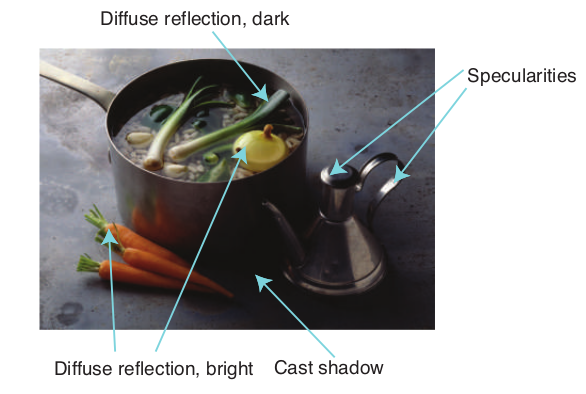
\includegraphics[width=0.6\textwidth]{figs/albedo.png} % Adicione uma imagem ilustrativa, se possível.
    \end{center}
\end{frame}

\begin{frame}{Aplicação em Visão Computacional}
    \begin{itemize}
        \item Superfícies são modeladas como tendo albedos difusos em RGB.
        \item Fontes de luz são representadas com intensidades RGB.
        \item Usando a lei do cosseno de Lambert, os valores RGB dos pixels são calculados para cada superfície.
        \begin{equation}
         I = \rho I_{0}\cos\theta
        \end{equation}
    \end{itemize}
\end{frame}

\begin{frame}{Constância de Cor}
    \begin{itemize}
        \item Observadores humanos conseguem ignorar variações de luz para inferir a cor verdadeira de uma superfície.
        \item Fenômeno conhecido como constância de cor:
        \begin{itemize}
            \item Permite ajustar a percepção em diferentes condições de iluminação.
        \end{itemize}
    \end{itemize}
\end{frame}

\subsection{Textura}
\begin{frame}{O que é Textura?}
    \begin{itemize}
        \item Em visão computacional, textura refere-se a padrões em superfícies que podem ser percebidos visualmente.
        \item Exemplos de texturas:
        \begin{itemize}
            \item Padrões de janelas em prédios.
            \item Pontos na pele de um leopardo.
            \item Pedras em uma praia.
        \end{itemize}
          \begin{center}
        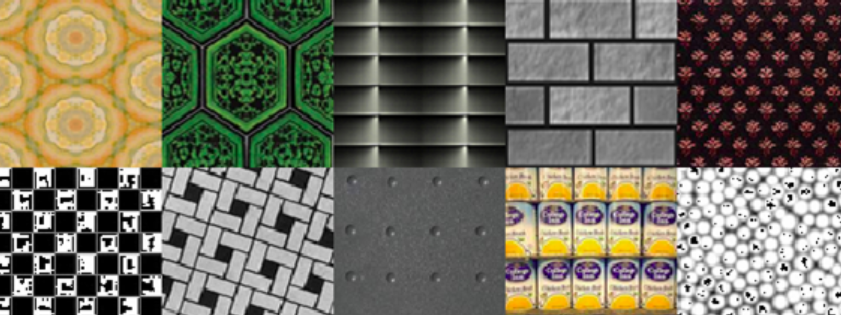
\includegraphics[width=0.6\textwidth]{figs/Texture_1.png} % Adicione uma imagem ilustrativa, se possível.
    \end{center}
    \end{itemize}
\end{frame}

\begin{frame}{Propriedades das Texturas}
    \begin{itemize}
        \item Textura é uma propriedade de uma região da imagem, não de pixels individuais.
        \item Representações úteis de textura:
        \begin{itemize}
            \item Devem ser invariantes a mudanças de iluminação.
            \item Devem capturar a orientação e padrões estatísticos de elementos repetitivos.
        \end{itemize}
    \end{itemize}
\end{frame}

\begin{frame}{Aplicações de Texturas}
    \begin{itemize}
        \item Identificação de objetos:
        \begin{itemize}
            \item Zebras e cavalos possuem formas similares, mas texturas distintas.
        \end{itemize}
 \begin{center}
        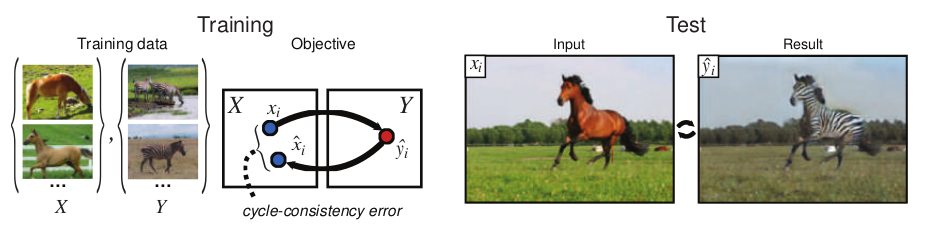
\includegraphics[width=1.\textwidth]{figs/Texture_3.png} % Adicione uma imagem ilustrativa, se possível.
    \end{center}
    \end{itemize}
\end{frame}

\begin{frame}{Construção de Representações de Textura}
    \begin{itemize}
        \item Calcula-se a orientação do gradiente em cada pixel de um patch da imagem.
        \item Caracteriza-se o patch por meio de histogramas de orientações:
        \begin{itemize}
            \item Estrias verticais produzem picos no histograma.
            \item Padrões mais complexos, como manchas, geram distribuições variadas.
        \end{itemize}
        \item Técnicas modernas utilizam redes neurais convolucionais para criar representações de texturas.
    \end{itemize}
\end{frame}

\section{Operações de Processamento de imagens}
\subsection{Bordas ou Arestas}
\begin{frame}{O que são bordas?}
    \begin{itemize}
        \item Bordas são mudanças significativas na intensidade de pixels em uma imagem.
        \item Representam:
        \begin{itemize}
            \item Descontinuidades de profundidade.
            \item Mudanças na orientação da superfície.
            \item Alterações na refletância.
            \item Sombras (descontinuidade na iluminação).
        \end{itemize}
        \item Objetivo: Reduzir a complexidade da imagem para uma representação compacta e abstrata.
    \end{itemize}
\end{frame}
\begin{frame}{O que são bordas?}
    \begin{center}
        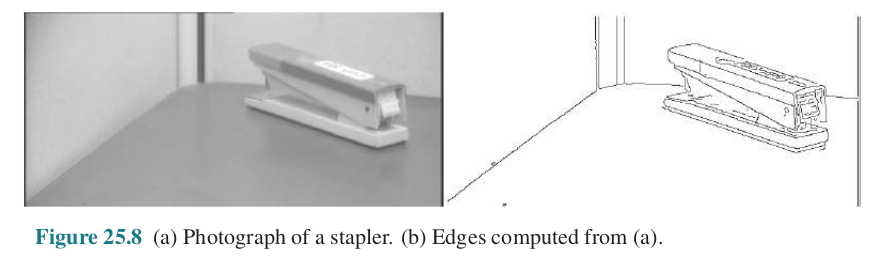
\includegraphics[width=1.\textwidth]{figs/Bordas.png} % Adicione uma imagem ilustrativa, se possível.
    \end{center}
\end{frame}



\begin{frame}{Detecção de bordas}
    \begin{itemize}
        \item Baseada na derivada da intensidade da imagem:
        \begin{itemize}
            \item Picos na derivada indicam bordas potenciais.
            \item Problemas: Ruído pode criar falsos positivos.
        \end{itemize}
        \item Solução:
        \begin{itemize}
            \item Suavizar a imagem antes de calcular a derivada.
            \item Uso de filtros Gaussianos para reduzir ruídos.
        \end{itemize}
    \end{itemize}

\end{frame}

\begin{frame}{}

       \begin{center}
        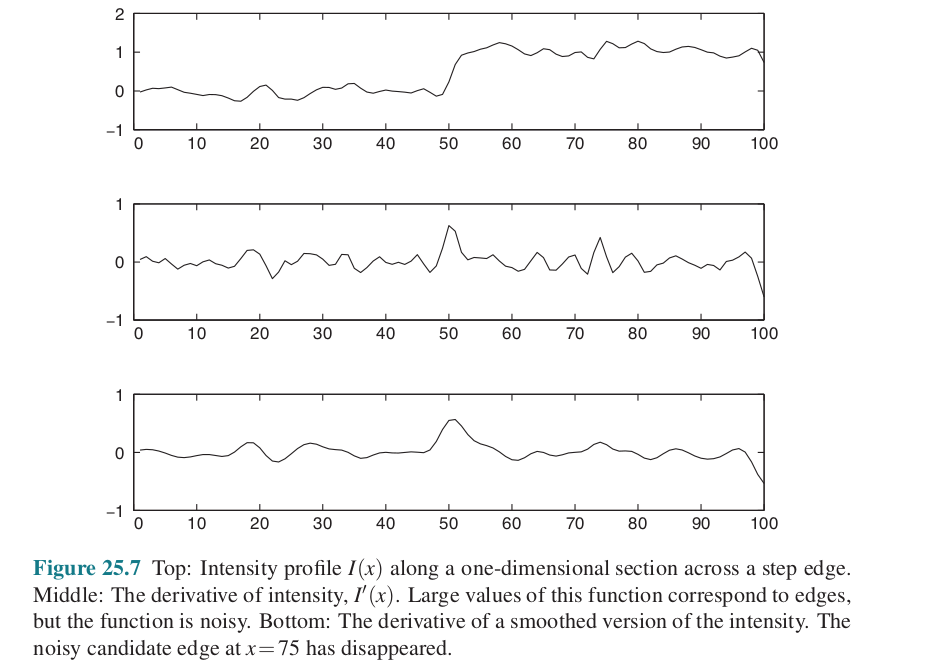
\includegraphics[width=1\textwidth]{figs/Bordas2.png} % Adicione uma imagem ilustrativa, se possível.
    \end{center}
\end{frame}

\begin{frame}{Gradiente da imagem}
    \begin{itemize}
        \item Representado por:
        \[
        \nabla I =
        \begin{pmatrix}
        \frac{\partial I}{\partial x} \\
        \frac{\partial I}{\partial y}
        \end{pmatrix}
        \]
        \item Bordas correspondem a pontos onde o gradiente é máximo.
        \item Orientação da borda é determinada pela direção do gradiente.
    \end{itemize}
\end{frame}

\begin{frame}{Vinculação de pixels de borda}
    \begin{itemize}
        \item Pixels detectados como bordas são agrupados para formar curvas contínuas.
        \item Critérios:
        \begin{itemize}
            \item Magnitude do gradiente é um máximo local.
            \item Orientações consistentes entre pixels vizinhos.
        \end{itemize}
    \end{itemize}
\end{frame}

\begin{frame}{Limitações e desafios}
    \begin{itemize}
        \item Ruídos ainda podem causar erros na detecção.
        \item Bordas detectadas podem não representar contornos reais de objetos.
        \item Processos subsequentes são necessários para correções e interpretações.
    \end{itemize}
\end{frame}

\subsection{Segmentação}
\begin{frame}{O que é Segmentação de Imagens?}
    \begin{itemize}
        \item Processo de dividir uma imagem em grupos de pixels similares.
        \item Propriedades utilizadas para segmentação:
        \begin{itemize}
            \item Brilho
            \item Cor
            \item Textura
        \end{itemize}
        \item Objetivo: Identificar regiões ou objetos na imagem.
    \end{itemize}
\end{frame}
\begin{frame}{Imagem Original}
  \begin{center}
        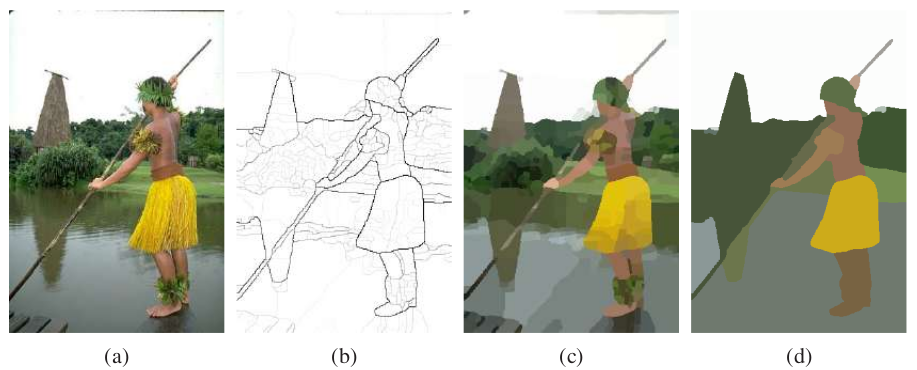
\includegraphics[width=1\textwidth]{figs/segmentacao.png}
    \end{center}
    \begin{description}
     \item[a)] Esta é a imagem de entrada, uma fotografia natural de uma pessoa em um ambiente externo.Ela serve como ponto de partida para o processo de segmentação.

    \end{description}
\end{frame}
\begin{frame}{Contornos de Bordas (Boundary Contours)}
  \begin{center}
        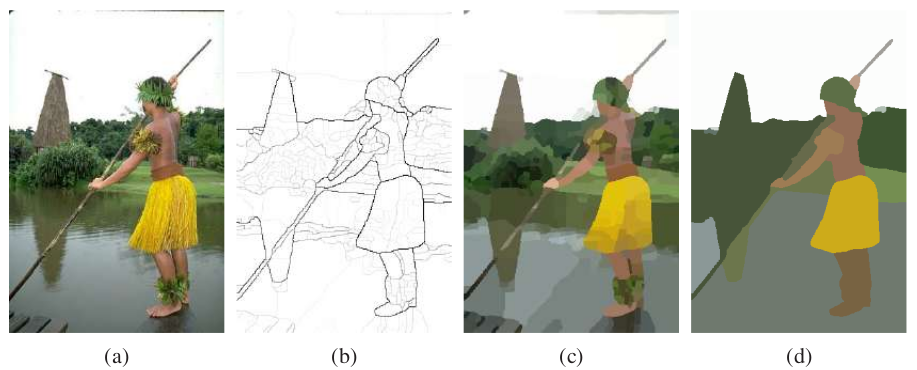
\includegraphics[width=0.8\textwidth]{figs/segmentacao.png}
    \end{center}
    \begin{description}
     \item[b)] Os contornos destacados representam mudanças significativas na intensidade de pixels (bordas). O valor $P_b$(probabilidade de borda) é usado para identificar os limites. Valores mais altos correspondem a bordas mais proeminentes, que aparecem mais escuras no resultado.

    \end{description}
\end{frame}

\begin{frame}{Segmentação em Regiões (Fine Partition)}
  \begin{center}
        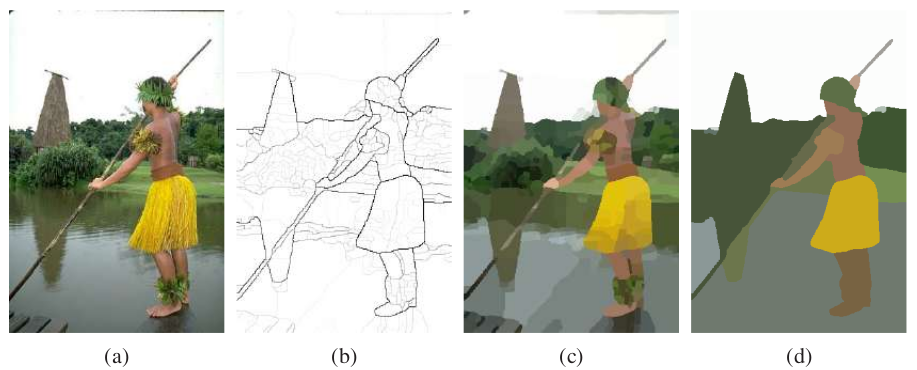
\includegraphics[width=0.8\textwidth]{figs/segmentacao.png}
    \end{center}
    \begin{description}
     \item[c)] A imagem é dividida em múltiplas regiões pequenas com base em propriedades como cor, brilho ou textura. Cada região é representada pela cor média dos pixels dentro dela. Este tipo de segmentação resulta em uma partição detalhada da imagem, onde cada detalhe é isolado.

    \end{description}
\end{frame}

\begin{frame}{Segmentação em Regiões Coarsas (Coarser Partition)}
  \begin{center}
        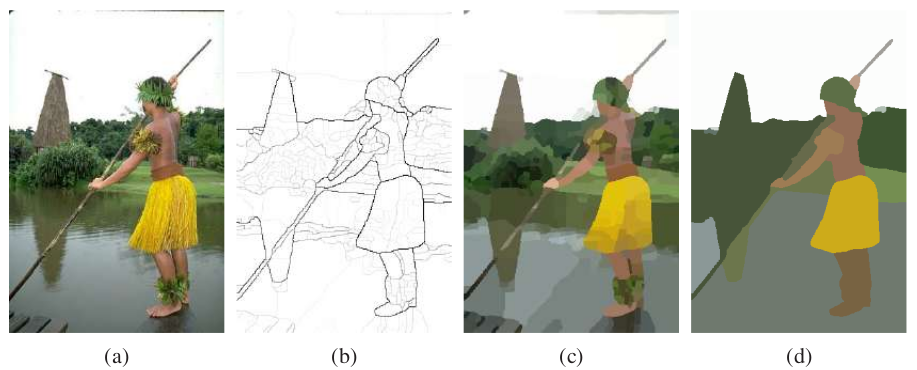
\includegraphics[width=0.8\textwidth]{figs/segmentacao.png}
    \end{center}
    \begin{description}
     \item[d)] Nesta etapa, as regiões finas da imagem são agrupadas em regiões maiores. O resultado é uma segmentação mais simples, que agrupa áreas similares e reduz o número total de regiões. Essa abordagem é útil para identificar estruturas maiores ou objetos completos na imagem.

    \end{description}
\end{frame}

\begin{frame}{Sobre Processo}
 \begin{itemize}
  \item A imagem ilustra o processo de segmentação, que começa com a detecção de contornos (b) e progride para dividir a imagem em pequenas regiões (c), culminando em uma segmentação mais simplificada (d).
  \item Este tipo de análise é crucial para aplicações como:
\begin{itemize}
 \item Reconhecimento de objetos.
  \item Compreensão da estrutura de imagens naturais.


\end{itemize}
\item A segmentação coarser (d) reduz a complexidade da imagem, tornando-a mais utilizável para modelos computacionais que trabalham com objetos completos.
 \end{itemize}

\end{frame}

\begin{frame}{Desafios na Segmentação}
    \begin{itemize}
        \item Apenas encontrar bordas não é suficiente.
        \item Exemplos:
        \begin{itemize}
            \item Bordas podem não corresponder aos contornos reais de objetos.
            \item Um tigre em meio à grama pode gerar bordas em cada listrado e folha, tornando difícil identificar o tigre como um todo.
        \end{itemize}
    \end{itemize}
\end{frame}

\begin{frame}{Abordagens para Segmentação}
    \begin{itemize}
        \item Foco em detecção de bordas:
        \begin{itemize}
            \item Baseado em probabilidade de uma borda existir em uma orientação específica.
            \item Usado para encontrar contornos, mas não garante regiões fechadas.
        \end{itemize}
        \item Foco em detecção de regiões:
        \begin{itemize}
            \item Agrupamento de pixels em regiões com base em suas propriedades (ex.: cor, brilho, textura).
            \item Exemplo: Método de particionamento de gráficos (Shi e Malik, 2000).
        \end{itemize}
    \end{itemize}
\end{frame}



\begin{frame}{Integração com Conhecimento de Alto Nível}
    \begin{itemize}
        \item A segmentação baseada em atributos locais (brilho, cor) não é suficiente para identificar corretamente todos os objetos.
        \item Necessidade de \textbf{conhecimento sobre os tipos de objetos} esperados em uma cena.
        \item Exemplo: Reconhecimento de um animal ou objeto específico em uma paisagem.
    \end{itemize}
\end{frame}

\begin{frame}{Etapas do Processamento de Imagens}
    \begin{itemize}
        \item \textbf{Baixo nível:}
        \begin{itemize}
            \item Transformação de imagem para outra imagem.
        \end{itemize}
        \item \textbf{Nível médio:}
        \begin{itemize}
            \item Transformação de imagem para características e atributos.
        \end{itemize}
        \item \textbf{Alto nível:}
        \begin{itemize}
            \item Transformação de características para reconhecimento.
        \end{itemize}
    \end{itemize}
\end{frame}

\begin{frame}{Baixo Nível}
   \begin{center}
        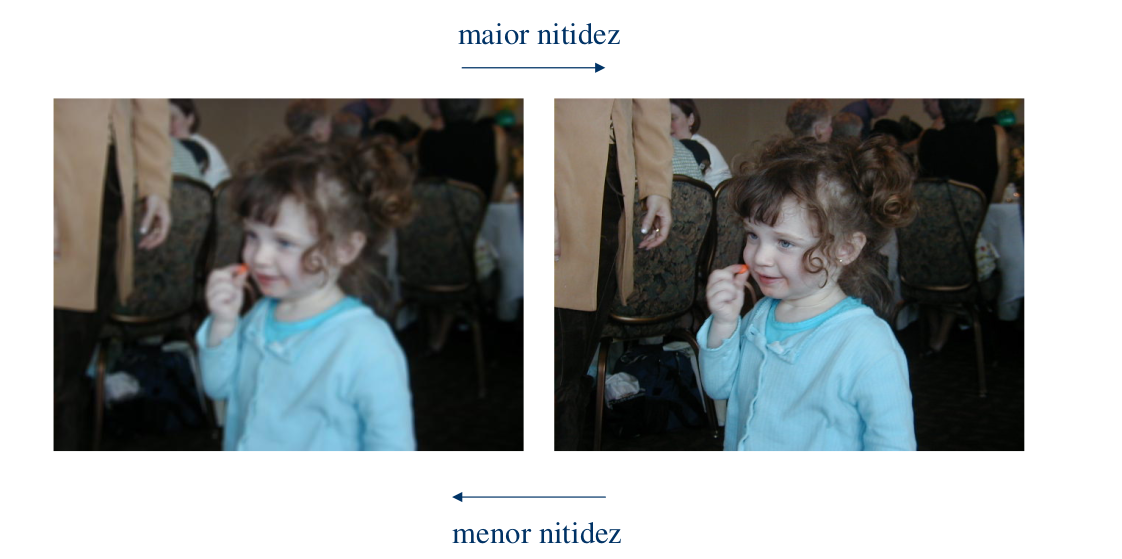
\includegraphics[width=1\textwidth]{figs/Baixo_nivel.png}
    \end{center}
\end{frame}

\begin{frame}{Médio Nível}
   \begin{center}
        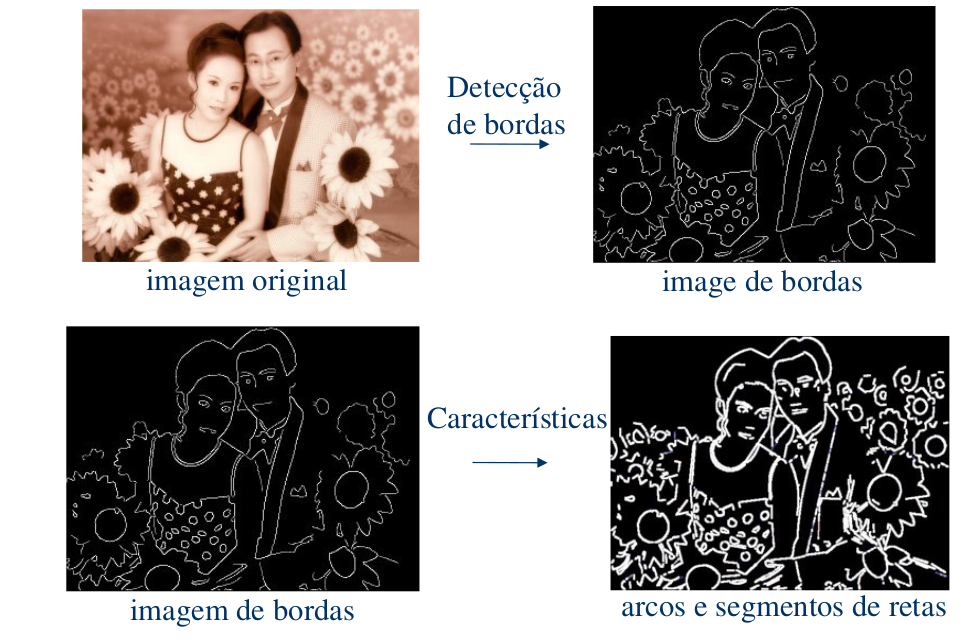
\includegraphics[width=1\textwidth]{figs/medio_nivel.png}
    \end{center}
\end{frame}

\begin{frame}{Médio Nível}
   \begin{center}
        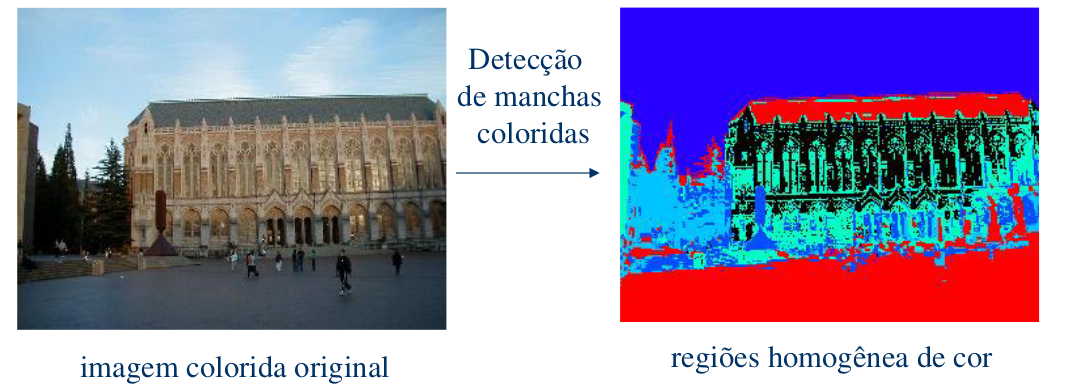
\includegraphics[width=1\textwidth]{figs/medio_nivel2.png}
    \end{center}
\end{frame}

\begin{frame}{Alto Nível}
   \begin{center}
        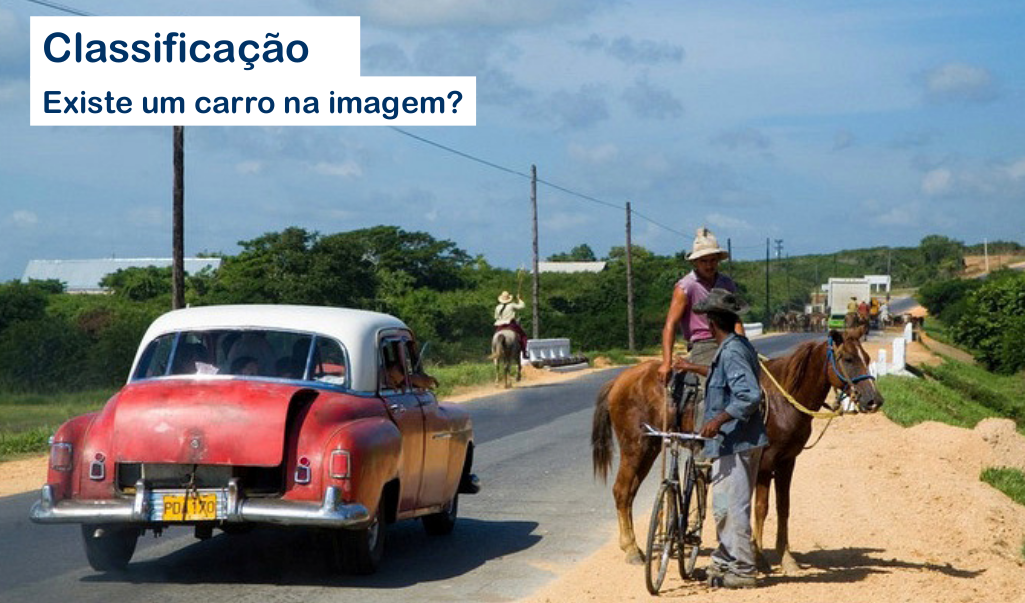
\includegraphics[width=1\textwidth]{figs/alto_nivel1.png}
    \end{center}
\end{frame}

\begin{frame}{Alto Nível}
   \begin{center}
        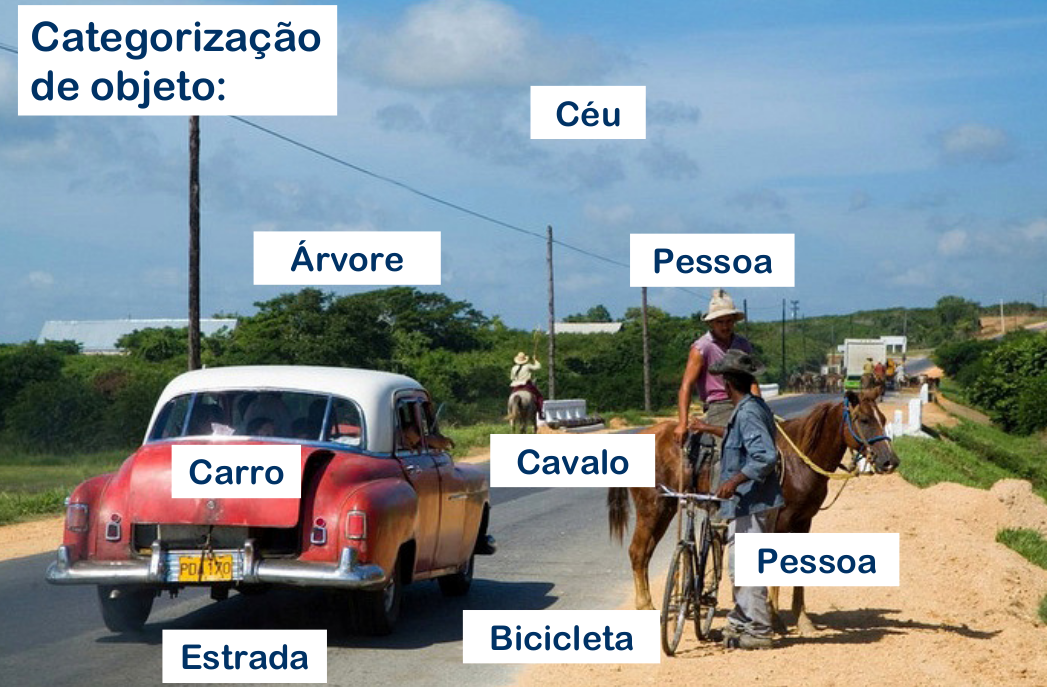
\includegraphics[width=0.9\textwidth]{figs/alto_nivel2.png}
    \end{center}
\end{frame}

\begin{frame}{Alto Nível}
   \begin{center}
        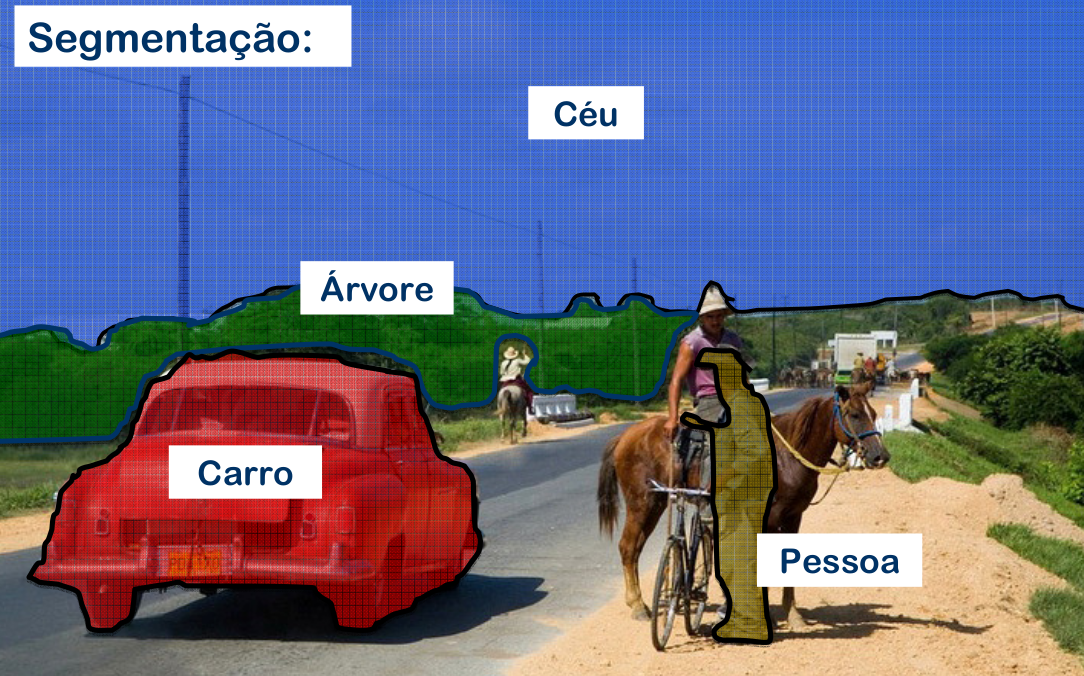
\includegraphics[width=0.9\textwidth]{figs/alto_nivel3.png}
    \end{center}
\end{frame}

\section{OpenCV}
\subsection{Introdução}
\begin{frame}
\centering
\Huge
\textbf{Aplicação de Visão Computacional}
\begin{center}
        
\includegraphics[width=0.2\textwidth]{figs/OpenCV.png}
    \end{center}
\end{frame}

\begin{frame}{Sobre OpenCV}
    \begin{itemize}
        \item \textbf{OpenCV (Open Source Computer Vision Library):}
        \begin{itemize}
            \item Biblioteca de software open source para visão computacional e aprendizado de máquina.
        \end{itemize}
        \item \textbf{Características:}
        \begin{itemize}
            \item Contém mais de 2500 algoritmos otimizados para tarefas como:
            \begin{itemize}
                \item Detecção de objetos.
                \item Montagem de imagens (Image Stitching).
                \item Classificação de ações humanas em vídeos.
            \end{itemize}
        \end{itemize}
        \item \textbf{Aplicações:}
        \begin{itemize}
            \item Utilizada amplamente por empresas (Google, Yahoo, Microsoft, etc.).
            \item Empregada em grupos de pesquisa e órgãos governamentais.
        \end{itemize}
        \item \textbf{Compatibilidade:}
        \begin{itemize}
            \item Interfaces disponíveis para C++, Python, Java e MATLAB.
            \item Suporte para Windows, Linux, Android e Mac OS.
        \end{itemize}
    \end{itemize}
\end{frame}

\begin{frame}{Instalação do OpenCV }
    \begin{itemize}
        \item Abra o Prompt de Comando e execute o seguinte comando:
        \end{itemize}
        \begin{center}
            \texttt{pip install opencv-python}\\
            \texttt{pip install opencv-contrib-python}
        \end{center}
    \begin{itemize}
        \item Guia detalhado disponível \href{https://github.com/opencv/opencv-python}{aqui}.
        \item Para incluir a biblioteca OpenCV no seu programa, use:
        \end{itemize}
        \begin{center}
            \texttt{import cv2}
        \end{center}
\end{frame}

\begin{frame}{Usando do OpenCV }
    \begin{itemize}
     \item Ler imagem
     \item Ler vídeo
    \end{itemize}

\end{frame}

\section{Referências Bibliográficas}
\begin{frame}[t,allowframebreaks]
\frametitle{Referências}
%\bibliographystyle{amsalpha}
%\bibliography{bibfile}
\begin{thebibliography}{*}

         \bibitem[A01]{A01} Chollet, F. (2021). Deep Learning with Python, Second Edition. Shelter Island, NY: Manning Publications.
        \bibitem[A02]{A02} Géron, A. (2019). Hands-On Machine Learning with Scikit-Learn, Keras, and TensorFlow. Sebastopol, CA: O'Reilly Media..
        \bibitem[A03]{A03} Russell, S., \& Norvig, P. (2021). Artificial Intelligence: A Modern Approach (4ª ed.). Hoboken, NJ: Pearson.
        \bibitem[A04]{A04}Moroney, L. (2020). AI and Machine Learning for Coders. Sebastopol, CA: O'Reilly Media.




\end{thebibliography}
\end{frame}
\section{}

%remover logo
\setbeamertemplate{logo}{}

\begin{frame}
\titlepage
\end{frame}

\end{document}
